
%****Header*****

\documentclass[%draft,
fleqn,											%richtet die Formel links aus, Einzug wird unten definiert
12pt,a4paper,
%twoside,openright,					%fuer einseitigen Druck diese beiden Optionen auskommentieren und unten ensprechende Kopfzeilenoption waehlen (bis ca 120 Seiten)
bibliography=totoc,listof=totoc,BCOR=5mm,
ngerman
%english
]{scrreprt}

%%%%%%%%%%%%%%%%%%%%%%%%%%%%%%%%%%%%%%%%%%%
%Textliches und sprachliches
%%%%%%%%%%%%%%%%%%%%%%%%%%%%%%%%%%%%%%%%%%%
\usepackage[T1]{fontenc}		% die beiden Packete geh�ren zusammen, um Umlaute und �hnliche deutsche "Sonderzeichen"
\usepackage[latin1]{inputenc} %direkt eingeben zu k�nnen
\usepackage[english]{babel}%kommt es zu einer Uebersetzung der sprachspezifischen Befehle im Dokument (�Inhaltsverzeichnis� statt �table of contents�, �Kapitel� anstelle von �chapter� usw.) und fuer korrekte Trennung wichtig
\usepackage{upgreek} 				%erlaubt die Eingabe von aufrechten griechischen Kleinbuchstaben
\pagestyle{headings} 				%schaltet die Kopfzeile ein. Die Option {headings} erzeugt die Nummer und den Namen des Kapitels
\usepackage{setspace} 			%enth�lt u.a. den Befehl \onehalfspacing, der daf�r sorgt, dass 1 1/2 Zeilen Abstand gelassen wird zwischen zwei Zeilen
\usepackage{rotating}
\usepackage{pdflscape}
\usepackage[euler]{textgreek}
%%%%%%%%%%%%%%%%%%%%%%%%%%%%%%%%%%%%%%%%%%%
%Verzeichnisse
%%%%%%%%%%%%%%%%%%%%%%%%%%%%%%%%%%%%%%%%%%%
\setcounter{secnumdepth}{2} %bestimmt, in welcher Tiefe Ueberschriften noch nummeriert werden. 5 Steht dafuer, dass alle Ueberschriften nummeriert werden
\setcounter{tocdepth}{1} 		%Bestimmt die Nummerierungstiefe im Inhaltsverzeichnis
\usepackage{cite}						%braucht man f�rs Literaturverzeichnis
\usepackage{bibgerm} 				%F�r die Literaturverzeichniserstellung auf deutsch
\usepackage{epstopdf}			% F�r eps Bilder
%%%%%%%%%%%%%%%%%%%%%%%%%%%%%%%%%%%%%%%%%%%
%Mathematisches
%%%%%%%%%%%%%%%%%%%%%%%%%%%%%%%%%%%%%%%%%%%
\usepackage{amssymb,amsfonts,amsmath} %Eingabehilfen f�r Formeln
\usepackage{siunitx} 				%erlaubt die Eingabe von Einheiten, so dass die Einheit und der Wert schoen zusammenstehen und nicht getrennt werden beim Zeilenumbruch.

%%%%%%%%%%%%%%%%%%%%%%%%%%%%%%%%%%%%%%%%%%%
%Bildtechnisches
%%%%%%%%%%%%%%%%%%%%%%%%%%%%%%%%%%%%%%%%%%%
\usepackage{graphicx} 			%um Bilder einzubinden
\usepackage[table]{xcolor}
\usepackage{float} 		%erlaubt mehr float Objekte (z.B. Bilder oder Tabellen) auf einer Seite
%\usepackage{subfig}				%wenn mehrere Bilder unter einer Caption zusammengefasst werden sollen
\usepackage[center,small,bf]{caption} %gibt die Optionen f�r das Verhalten der Bildunterschriften (caption) an, muss nach Paketen wie subfig, float, rotating eingebunden werden

%%%%%%%%%%%%%%%%%%%%%%%%%%%%%%%%%%%%%%%%%%%
%Fuss- und Kopfzeilendefinition
%%%%%%%%%%%%%%%%%%%%%%%%%%%%%%%%%%%%%%%%%%%
\usepackage{fancyhdr}
\fancyhead{}
\fancyfoot{}
\renewcommand{\headrulewidth}{0.5pt}

%%% zweiseitiges Seitenlayout
%\fancyhead[EL, OR]{ \thepage}
%\fancyhead[EC]{\textsl{\leftmark}}
%\fancyhead[OC]{\textsl{\rightmark}}
%%% Ende: zweiseitiges Seitenlayout

%%% einseitiges Seitenlayout
\fancyhead[R]{ \thepage}
\fancyhead[C]{\textsl{\leftmark}}
%%% Ende: einseitiges Seitenlayout

\pagestyle{fancy}

\renewcommand{\chaptermark}[1]{%
\markboth{\thechapter\ #1}{}}

\renewcommand{\sectionmark}[1]{%
\markright{\thesection\ #1}}

%------------------------------------------------------------------------------
%Bis hierhin darf der Header nur in Ruecksprache mit dem Betreuer geaendert werden.
%------------------------------------------------------------------------------

%%%%%%%%%%%%%%%%%%%%%%%%%%%%%%%%%%%%%%%%%%%
%Definitionen f�r siunitx-Paket
%wird nur in deutscher Version benoetigt
%%%%%%%%%%%%%%%%%%%%%%%%%%%%%%%%%%%%%%%%%%%
\sisetup{locale=DE} 			%macht, dass statt Punkt ein Komma als Dezimaltrenner verwendet wird
\sisetup{%
  list-final-separator = { \translate{and} },
  range-phrase = { \translate{to (numerical range)} }
} 												%macht dass in Liste und Range die Woerter richtig uebersetzt werden

%%%%%%%%%%%%%%%%%%%%%%%%%%%%%%%%%%%%%%%%%%%
%Einbinden mehrseitiger PDFs oder Ausschnitte daraus
%%%%%%%%%%%%%%%%%%%%%%%%%%%%%%%%%%%%%%%%%%%
%\usepackage{calc}
%\usepackage{eso-pic}
%\usepackage{everyshi}
%\usepackage{pdfpages}

%%%%%%%%%%%%%%%%%%%%%%%%%%%%%%%%%%%%%%%%%%%
%Fuer das Erstellen von Bildern aus Matlab mit \psfragfig
%%%%%%%%%%%%%%%%%%%%%%%%%%%%%%%%%%%%%%%%%%%
%Fuer die Nutzung von \psfragfig muessen die Bilder mit Hilfe des figures_fuer_latex.m erzeugt werden -- es muss dem Complier noch das Argument "-shell-escape" uebergeben werden (bei Texniccenter Alt+F7)
%\usepackage{pstool}
\usepackage[crop=pdfcrop]{pstool} %verschmaelert die Raender der Abbildung
%\usepackage[cleanup={}]{pstool} 	 %log-Datei bleibt erhalten: zum Debuggen

%%%%%%%%%%%%%%%%%%%%%%%%%%%%%%%%%%%%%%%%%%%
%Fuer den Import von Bildern aus Inkscape
%%%%%%%%%%%%%%%%%%%%%%%%%%%%%%%%%%%%%%%%%%%
%\graphicspath{{figures/}}
%\newcommand{\executeiffilenewer}[3]{%
%\ifnum\pdfstrcmp{\pdffilemoddate{#1}}%
%{\pdffilemoddate{#2}}>0%
%{\immediate\write18{#3}}\fi%
%}
%\newcommand{\includesvg}[1]{%
%\executeiffilenewer{#1.svg}{#1.pdf}%
%{inkscape -z -D --file=#1.svg %
%--export-pdf=#1.pdf --export-latex}%
%\input{#1.pdf_tex}%
%}

%%%%%%%%%%%%%%%%%%%%%%%%%%%%%%%%%%%%%%%%%%%
%Fuer TpX
%Mit TpX koennen unter Window recht einfach Diagramme erstellt werden
%%%%%%%%%%%%%%%%%%%%%%%%%%%%%%%%%%%%%%%%%%%
%\usepackage{color,ifpdf,graphicx}
%\ifpdf %if using PDFTeX in PDF mode
%  \DeclareGraphicsExtensions{.pdf,.png,.mps}
%\else %if using TeX or PDFTeX in TeX mode
%  \DeclareGraphicsExtensions{.eps,.bmp}
%  \DeclareGraphicsRule{.emf}{bmp}{}{}% declare EMF filename extension
%  \DeclareGraphicsRule{.png}{bmp}{}{}% declare PNG filename extension
%  \usepackage{pstricks}%variant: \usepackage{pst-all}
%\fi
%\usepackage{pgf,epic,bez123,floatflt,wrapfig}

%%%%%%%%%%%%%%%%%%%%%%%%%%%%%%%%%%%%%%%%%%%
%Neu-/Umdefinitionen
%%%%%%%%%%%%%%%%%%%%%%%%%%%%%%%%%%%%%%%%%%%
\usepackage[pdfborder={0 0 0}, breaklinks=true]{hyperref} %muss als letztes Paket eingebunden werden, verlinkt Referenzen, so dass im pdf direkt zu der Stelle gesprungen wird

%%%%%%%%%%%%%%%%%%%%%%%%%%%%%%%%%%%%%%%%%%%
%Neu-/Umdefinitionen
%%%%%%%%%%%%%%%%%%%%%%%%%%%%%%%%%%%%%%%%%%%

\newcommand{\sfs}{SF$_6$} 
%% ----------------------------------------------------------------
% Aus AMS
% ----------------------------------------------------------------

\newcommand{\titlestring}{{Berechnung und Reduktion der tonalen
Ger�uschemission von Hochspannungsfreileitungen}}

\newcommand{\UnterTitlestring}{{Berechnung und Massnahmen zu deren
Reduktion}}

\newcommand{\DissNummer}{{17408}}
\newcommand{\degreestring}{{Doktor der Wissenschaften}}
\newcommand{\authorstring}{{Ulrich Straumann}}
\newcommand{\acadtitlestring}{{Dipl.-Phys. Universit�t Z�rich}}
\newcommand{\dateofbirthstring}{{11. Januar 1975}}
\newcommand{\citizenstring}{{Fehren SO und Oberg�sgen SO}}
\newcommand{\examinerstring}{Prof. Dr. K. Fr�hlich}
\newcommand{\coexaminerstring}{Prof. Dr. E. Gockenbach, Korreferent \\ Dr. K. Heutschi}

\EndPreamble
\begin{document}

	\pagenumbering{roman} 		%Schaltet die Seitenzahlen auf roemische Zahlen

%	\begin{titlepage}
\setlength{\baselineskip}{8mm}
{\large\noindent DISS.\ ETH Nr.\ \DissNummer}
\vfill
\begin{center}
  {\def\\{\linebreak}
  \huge\bf\titlestring}
\end{center}
\vfill
\begin{center}
  \large ABHANDLUNG \linebreak
  zur Erlangung des Titels \linebreak
  \degreestring
\end{center}
\vspace{0.5\fill}
\begin{center}
  \large der \linebreak
  EIDGEN�SSISCHEN TECHNISCHEN HOCHSCHULE \linebreak
  Z�RICH
\end{center}
\vspace{0.5\fill}
\begin{center}
  \large vorgelegt von \vspace{5mm}  \linebreak %NK
  \textsc{\authorstring} \vspace{5mm} \linebreak  %NK
  \acadtitlestring \linebreak
  geboren am \dateofbirthstring \linebreak
  von \citizenstring
\end{center}
\vspace{0.5\fill}
\begin{center}
  \large Angenommen auf Antrag von: \linebreak
  \examinerstring, Referent \linebreak
  \coexaminerstring, Korreferent
\end{center}
\vspace{0.5\fill}
\begin{center}
  \large\number\year
\end{center}
\end{titlepage}

	

%**** Titelseite *****

\pagestyle{empty}

\begin{figure}
    \begin{minipage}[b]{0.5\linewidth}
        \includegraphics[width=0.8\textwidth]{figures/ethlogo}
    \end{minipage}
    \hfill
    \begin{minipage}[b]{0.45\linewidth}
        \flushright
        \textbf{High Voltage Laboratory}\\
        \vspace{3mm}
        Prof. Dr. Christian Franck
    \end{minipage}
\end{figure}


\begin{flushright}
    \textit{ETH Z�rich\\
    Physikstr. 3, ETL\\
    8092 Zurich\\
    Switzerland}
\end{flushright}

\phantom{u}
\vspace{1.5cm}
\Huge{\sc TITEL}
\vspace{1.5cm}

\Large
SEMESTERARBEIT/MASTERARBEIT\\

\vspace*{5cm} \large
Vorname Name

Email-Adresse

\normalsize

\vspace{1.5cm}

Betreuer: Name Betreuer

Semester 
	\cleardoublepage					%notwendig, damit keine Seitenzahl auf Titelseite

%%%%%%%%%%%%%%%%%%%%%%%%%%%%%%%%%%%%%%%%%%%%%%%%%%%%%%%%%%%%%%%%%%%%%%%%%%%%%%%%
%Vorspann
%%%%%%%%%%%%%%%%%%%%%%%%%%%%%%%%%%%%%%%%%%%%%%%%%%%%%%%%%%%%%%%%%%%%%%%%%%%%%%%%
	\pagestyle{fancy}
	
	
<<<<<<< HEAD
\begin{center}
  \makebox[\textwidth]{\includegraphics[width=\paperwidth, height=\paperheight]{figures/Project_Definition_Philipp_Deuschle_HS15.pdf}}
=======
\chapter*{Aufgabenstellung}



\includegraphics{figures/Project_Definition_Philipp_Deuschle_HS15.pdf}
>>>>>>> 0d939384617ec4e70e21752a52b662e06c59e28a

	
\chapter*{Kurzfassung}

Der Zweck der Kurzfassung ist, die wesentlichen Informationen und Konsequenzen aus der Arbeit dem Leser in kurzer Form anzubieten. Sie soll daher folgendermassen aufgebaut werden:
\begin{enumerate}
    \item Problemstellung (inkl. Hintergrund)
    \item Innovation / Neue Elemente
    \item Methode / L�sungswege
    \item Wesentliche Resultate
    \item Schlussfolgerungen
    \item Konsequenzen f�r die Fachwelt, das Projekt oder weitere Arbeiten
\end{enumerate} 
%	\input{text/Abstract}

	\tableofcontents 				%erzeugt das Inhaltsverzeichnis

	\cleardoublepage 				%notwendig, damit arabische Nummerierung erst beim ersten Kapitel beginnt
	\pagenumbering{arabic} 	%Schaltet die Seitenzahlen auf arabische Zahlen
%	\onehalfspacing

%%%%%%%%%%%%%%%%%%%%%%%%%%%%%%%%%%%%%%%%%%%%%%%%%%%%%%%%%%%%%%%%%%%%%%%%%%%%%%%%
%Hauptteil
%%%%%%%%%%%%%%%%%%%%%%%%%%%%%%%%%%%%%%%%%%%%%%%%%%%%%%%%%%%%%%%%%%%%%%%%%%%%%%%%

	\input{text/abstract}
	%
	
\chapter{Introduction}
Power electronics systems, especially converters, lead to a more complex electrical field stress in insulation material of energy transmission systems as it introduces pulses (>1 kV) with high slew rates (>$10 \frac{kV}{\mu s}$) and high repetition frequencies (> 1 kHz) superimposed on low frequencies (50 Hz) or DC. The latter can cause enhanced partial discharges (PD) in the insulation system, i.e. a breakdown of a part of the insulation system. \cite{TransformerEngineering}. However, there are already effects below partial discharge inception that are not well understood, yet. They do as well result in an accelerated aging of the insulation due to the sustained application of the converter pulses. 
\newline

\begin{figure}[!ht]
  \begin{minipage}{0.5\textwidth}
  

  
  \centerline{\includegraphics[height=0.2\textheight]{figures/intro/cad_epoxy}}
\caption{CAD model of epoxy specimen used for measurements}
	\label{fig.specimen}
	
	  \end{minipage}
	    \begin{minipage}{0.5\textwidth}
	  
  \centerline{\includegraphics[height=0.2\textheight]{figures/intro/photo_epoxy2}}
\caption{Photo of Epoxy specimen used for measurements of the partial discharges. \protect\footnotemark}
	\label{fig.specimenphoto}
	  
	   \end{minipage}
\end{figure}
\footnotetext{{Both figures provided by Raphael F\"arber}}
In a new approach, a quantification of the pre-breakdown modification within the insulation material should be obtained with the use of an online monitoring of the dielectric permittivity for several harmonics of the applied pulse spectrum \cite{FaerberMVISS}.
The first part of this semester project is aimed at getting the dielectric permittivity by once measuring the capacity of the specimen shown in figure \ref{fig.specimen} in conjuction with numerical field simulations. When using a specimen after manufacturing it is assumed that it's dielectric permittivity is always the same. In order to be able to determine the distance of the two electrodes a reference measurement of the actual distance and the permittivity for two samples is made and a look-up table containing the electrode distance for different vacuum capacities is created. 

The second part of the project is the investigation of the suitability of current transformers in dielectric spectroscopy. With regard to the small capacitive current through the sample, it is the aim to prove or disprove that a current transformer does not deteriorate the signal in a way that makes dielectric spectroscopy is impossible. 



	%
	\chapter{Theory}
\section{Debye model}
The polarization effects in a dielectric material can be characterized by the relative permittivity and the dielectric loss factor. 
For linear materials the polarization can be described by a network model. The Debye-ansatz assumes that the rate of change $ dP_i/dt$ is of the remaining difference between the polarization $P_i(t)$ and the polarization at infinity $P_i(\infty$) is proportional. This results in an exponential decay of the polarization function that towards $P_i(\infty)$. This exponential decay can be modeled with a time constant of a resistor and a capacitor in series ($\tau=R_i \cdot C_i$). 

\subsection{Derivation of maximum tan($\delta$)}
The aim of this section is to derive the formula for the maximum tan($\delta$) of the Debye model in order to adjust its value to a disired one.
\begin{equation}
\epsilon_{eff}^* (\omega) = \frac{C^*(\omega)}{C_0}
\end{equation}

\begin{equation}
\epsilon^* = \epsilon_r-j \cdot \epsilon_r''
\end{equation}


\begin{equation}
\epsilon'_r = \epsilon_{\infty} + \frac{\epsilon_{stat}-\epsilon_{\infty}}{1+(\omega \cdot \tau )^2}
\end{equation}

\begin{equation}
\epsilon''_r = \omega \cdot \tau \cdot \frac{\epsilon_{stat}-\epsilon_{\infty}}{1+(\omega \cdot \tau )^2}
\end{equation}

The loss tangents are given by:
\begin{equation}
tan (\delta) = \frac{\kappa + \omega \cdot \epsilon_0 \cdot \epsilon _r ''}{\omega \cdot \epsilon_0 \cdot \epsilon _r '}
\end{equation}

\begin{equation}
tan (\delta_{L}) = \frac{\kappa}{\omega \cdot \epsilon_0 \cdot \epsilon_r'} \newline
\end{equation}

\begin{equation}
tan (\delta_{pol}) = \frac {\epsilon_r'' } {\epsilon_r'}
\end{equation}


We are measuring in the frequency domain from $10^{-6}$ Hz to $10^{11}$ Hz 

\begin{equation}
\epsilon^*(\omega) = \frac{1}{j \omega  Z^*(\omega) C_0}
\end{equation}

\begin{equation}
Z_0(\omega)=[\frac{1}{R_\infty}+\frac{1}{R_i+\frac{1}{j \omega C_i}}+j \omega C_0]^{-1} = [\frac{1}{R_\infty}+\frac{j \omega C_i}{j\omega R_i  C_i+1}+j \omega C_0]^{-1}
\end{equation}

\begin{equation}
\epsilon^*(\omega)= \frac{[\frac{1}{R_\infty}+\frac{j \omega C_i}{j\omega C_i R_i  +1}+j \omega C_0]}{j \omega C_0} = \frac{1}{j \omega C_0 R_\infty}+ \frac{C_i/C_0}{j\omega C_i R_i  +1}+1
\end{equation}

We split this term up into real and impaginary part 

\begin{equation}
\epsilon_r' = 1+ \frac{C_i/C_0}{\omega^2 C_i^2 R_i^2 +1}
\end{equation}

\begin{equation}
\epsilon_r'' = -j \left(\frac{1}{\omega C_0 R_\infty}+\frac{\omega C_i^2 R_i / C_0}{\omega^2 C_i^2 R_i^2 +1} \right)
\end{equation}

\begin{equation}
tan(\delta) = tan(\delta_L) + tan( \delta_Pol) = \frac{\omega^2 \tau^2+1}{\omega C_0 R_\infty (2+ \omega^2 \tau^2)}=\frac{\omega \tau \Delta \epsilon}{\epsilon_{stat} + \omega^2 \tau^2}
\end{equation}

\begin{equation}
\frac{\partial tan(\delta)}{ \partial \omega} = \frac{[\omega C_0 R_\infty (2+\omega^2 \tau^2)]\cdot 2 \omega \tau^2 - (\omega^2 \tau^2 +1) [C_0 R_\infty (2+3 \omega^2 \tau^2)  }{[\omega C_0 R_\infty (2+\omega^2 \tau^2)]^2}+ \frac{\tau \Delta \epsilon [\epsilon_{stat} + \omega^2 \tau^2] - 2 \omega \tau^2 [\omega \tau \Delta \epsilon]}{[\epsilon_{stat} +\omega^2 \tau^2]}
\end{equation}

Um das Maximum von tan($\delta_{pol}$) zu finden wird der zweite Term in der Ableitung 0 gesetzt.

\begin{equation}
\tau \Delta \epsilon [\epsilon_{stat} + \omega^2 \tau^2] -2\omega \tau^2 [\omega \tau \Delta \epsilon] = 0
\end{equation}
\begin{equation}
\omega^2 (\tau^3 \Delta \epsilon -2 \tau^3 \Delta \epsilon) = - \tau \Delta \epsilon \cdot \epsilon_{stat}
\end{equation}
\begin{equation}
\omega^2 = \frac{\tau \Delta \epsilon \epsilon_{stat}}{\tau^3 \Delta \epsilon}
\end{equation}
\begin{equation}
\omega = \sqrt{\frac{\epsilon_{stat}}{\tau^2}}
\end{equation}
\begin{equation}
\tan(\delta_L)_{max} = \frac{\epsilon_{stat} \Delta\epsilon}{2\epsilon_{stat}} = \frac{1}{2} \frac{\Delta \epsilon}{\sqrt{\epsilon_{stat}}}
\end{equation}


\section{Fourier Coefficients of trapezoidal pulse  train }
\begin{equation}
 U_n = \frac{2 U_0}{j \omega_n T} [e^{\frac{j \omega_n \tau}{2}} sinc{\frac { \omega_n \tau_r }{2}} -e^{\frac{-j \omega_n \tau}{2}} sinc{\frac{ \omega_n \tau_f}{2}}]
\end{equation}
 
System Analysis: 
 
 
\begin{equation}
 \tau_r = 0.5e^{-6 }
  \end{equation}
  \begin{equation}
 \tau_f = 0.1e^{-6}
  \end{equation}
 \begin{equation}
\tau= 1e^{-6}
 \end{equation}
 
Slopes of the curves: \newline
-1 on loglog plot after $\frac{2}{\tau}$ \newline
-2 on loglog plot after $\frac{2}{\tau_r}$




	%
	\chapter{Methods}
\section{Part 1}
\subsection{Simulation of vacuum capacitance} 
The dependency of the vacuum capacity $C_0$ has to be simulated numerically for the high-voltage setup as well as for the low-voltage setup. 
\begin{figure}[htbp]
	\centering
	\includegraphics{figures/COMSOL_Beispielbild.jpg}		
	\caption[Kurze Abbildungsbeschreibung]{Field simulation of the low-voltage test cell (0.5 mm electrode distance)} \ref{sec.analysecurrent}
	\label{fig.waveforms}
\end{figure}
 
There are several systematic errors that influence the vacuum capacity. One factor is the air gap between the wall of the low-voltage setup and the specimen. This air gap is unavoidable in order to be able to remove the specimen from the pouring setup. This air gap should theoretically be 0.5 mm, but it is expected to vary in worst-case between 0 mm and 1 mm. The lookup table of d based on $C_0$ is based on an air gap of 0.5 mm, therefore the deviation from this value has to be investigated. 
Another systematic error is the deviation of the height of the specimen. During  the pouring process the height of the specimen cannot be . The maximum deviation is expected to be $\pm$ 0.5 mm. This deviation might occur during the production process of each new specimen. Thus, if the electrode distance of a specimen should be estimated by the method described in !!! this 
A third influence is the 

\section{Part 2}
\section{Signal analysis of the Debye model}

In order to emulate different dielectrica with their own respective dielectric loss tangent, different combinations of circuit elements were used. Each different circuit accounts for another loss tangent with respect to frequency. With the objective to assess the performance of the current transformer, reasonably high values for the $tan\left(\delta\right)$ were assumed (i.e. 0.05 to 0.2) since a lower loss tangent would require a higher resolution on the part of the current measurement.


\begin{figure}[htbp]
	\centering
	\includegraphics{figures/COMSOL_Beispielbild.jpg}		
	\caption[Kurze Abbildungsbeschreibung]{Electron drift currents in Ar at 30 Td and in CO$_2$ at 65 Td, the latter was divided by 10 and shifted by 0.2 $\mu$s. Dotted lines are averages of measured waveforms, solid lines are fits of Eq. XX. $T$ marks the electron transit time, and the markers $T_1$ to $T_3$ are explained in section.} \ref{sec.COMSOL_Beispielbild}
	\label{fig.waveforms}
\end{figure}


\subsection{Design of a holder for the Debye Equivalent Circuit}
For a lossy medium the Debye Network consists at least of a vacuum capacity $C_0$ and the term for the charging of the additional capacitance. There might be . Thus, it is reasonable to design a holder for the network that can hold three strands with two components each. Moreover, it has to fit into the low-voltage and high-voltage test cell. 

\begin{figure}
\includegraphics[width=\textwidth]{figures/Method/CAD_MODEL/Gesamtanordnung.jpg}
\end{figure}
\newpage

\begin{sidewaysfigure}
\includegraphics[width=0.99\textwidth]{figures/Gesamtanordnung.pdf}
    \caption{Property profile of the diverse library compared to the compound pool.}
    
   \end{sidewaysfigure}	
\newpage
    

\subsection{Measurement of the textepsilon and the tan(textdelta) for the Debye model}

The aim is to have a current flwoing though the Debye model in the low-voltage setup that is oft the same order as a current in the high voltage-setup. In order to have a comparable current for a voltage that is $1/1000$ of the high-voltage setup a capacitance $C_0$ for the Debye is selected 1000 times higher than the Capacitance of the samples. As the sample has a capacitance of 3.44 pF its equivalent $C_0$ in the debye-model is 3.3 nF. In order to get a tan($\delta$) of !!! $R_i$ is chosen as and $C_i$ is chosen as .
\begin{figure}
	\includegraphics{figures/Method/debye-modell.jpg}	
	\caption{Debye model for tan($tan(\delta)$)= }	
\end{figure}






\subsection{Integrator}
\subsection{Advantages of using an integrator}
As the used 16-bit DAC has a limited resolution it is advantageous to use an integrator in order to spread the frequencies of the signal over a larger timescale. This makes it possible to detect the different frequencies more accurately with the same DAC. 
A second reason to make use of an integrator is due to the fact that it adds an additional factor of $1/f$ to the Fourier spectrum of the output voltage signal. As the Fourier spectrum of the input signal is as well characterized by a $1/f$ decrease the integrator transforms the pulse signal back to a trapezoidal signal with a $1/f$-dependency in the Fourier spectrum. Since a $1/f$ dependency in the output signal is preferable to a constant Fourier spectrum due to better resolution for the first harmonic, the integrator improves the measurement as well. 
\subsection{Design of integrator}
The integrator should have two functions. On the hand side it should integrate signal on the other hand it should amplify the signal by a factor of 1000. This is due to the fact small below-PD-currents ($\sim$mA) should be measured. With a CT-sensitivity of $1V/A$ an amplification of 1000 is reasonable to use the range of measurable inputs of $\pm$ 10 V. These requirements can be achieved by a non-inverting integrator. 

\begin{sidewaysfigure}
\includegraphics[width=0.99\textwidth]{figures/Method/integrator/PCB_Integrator.png}
    \caption{Property profile of the diverse library compared to the compound pool.}
    
    \end{sidewaysfigure}	
    
    
    \newpage
    
    	\begin{sidewaysfigure}
\includegraphics[width=0.99\textwidth]{figures/Method/integrator/schematic.jpg}
 \caption{Property profile of the diverse library compared to the compound pool.}
  \end{sidewaysfigure}	

The integrator has the following theoretical transfer function.

\begin{figure}

\includegraphics[width=\textwidth]{figures/Method/integrator/transferfunction_int.jpg}





\caption[Kurze Abbildungsbeschreibung]{Bode plot of an integrator } \ref{sec.Bodeplot}
\end{figure}
	



\subsection{Protective Clamping Capability of the current transformer}


	%
	
\chapter{Results}
\section{Simulation of Capacitance values}
\subsection{Comparision of Capacitance in the simulation with a sphere geometry}
The simulation of the capacitance for the cylindric geometry as a function of different distances with COMSOL leads to the following figure.The simulation of two spheres as well as the approximation formula result in a general shift which is due to the fact that it is a three electrode arrangement as the wall of the low-voltage introduces a new capacitance between the upper electrode and the wall which is not affected by the distance variation. This results in a reduction of the capacitance compared to the two spheres geometry. Thus, the simulated values for the low voltage test cell seem reasonable if one compares them to the results of the capacitance between two spheres. \newline 



\begin{figure}[]
	\centering
	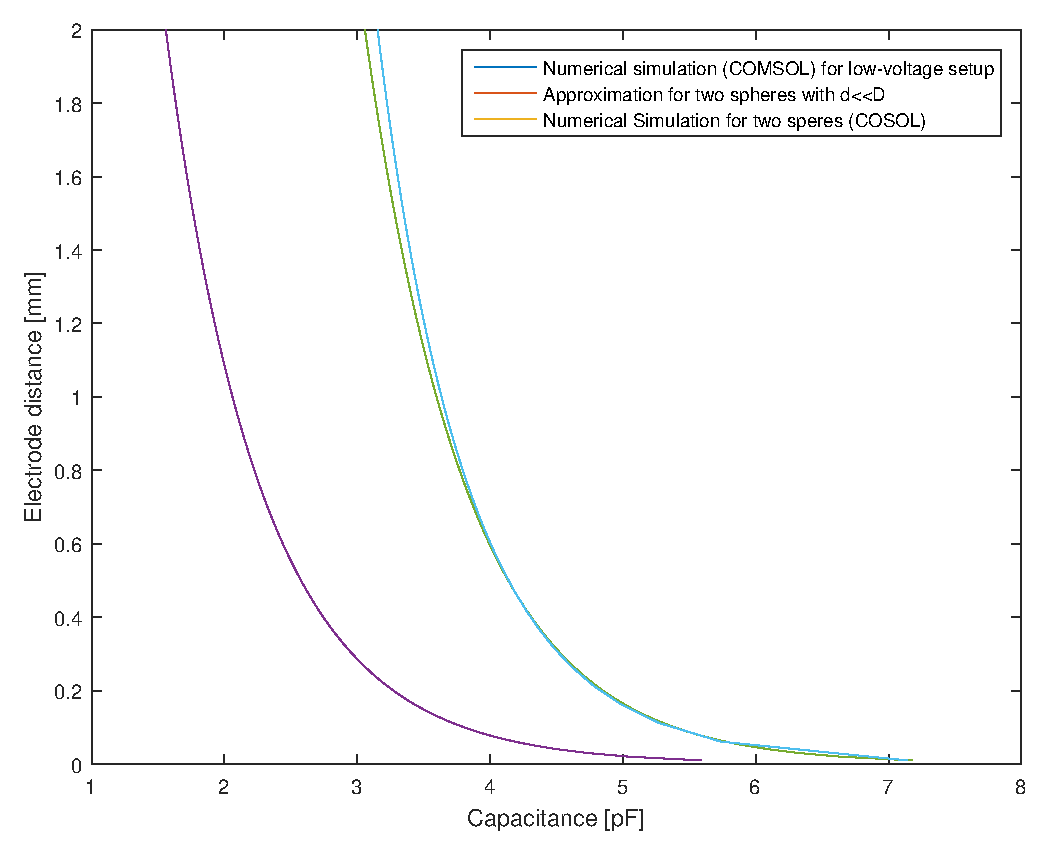
\includegraphics[scale=1]{figures/Comparison_Low_voltage_Two_spheres}		
	\caption[Kurze Abbildungsbeschreibung]{Dependency of the electrode distance on the capacitance for the low voltage setup and two spheres $\epsilon = 3.5$ } 
	\label{fig.waveforms}
\end{figure}

\section{Complex effective permittivity}
\subsection{}

\chapter{Results}
\section{Simulation of Capacitance values}
\subsection{Comparision of Capacitance in the simulation with a sphere geometry}
The simulation of the capacitance for the cylindric geometry as a function of different distances with COMSOL leads to the following figure.The simulation of two spheres as well as the approximation formula result in a general shift which is due to the fact that it is a three electrode arrangement as the wall of the low-voltage introduces a new capacitance between the upper electrode and the wall which is not affected by the distance variation. This results in a reduction of the capacitance compared to the two spheres geometry. Thus, the simulated values for the low voltage test cell seem reasonable if one compares them to the results of the capacitance between two spheres. \newline 


\begin{figure}[htbp]
	\centering
	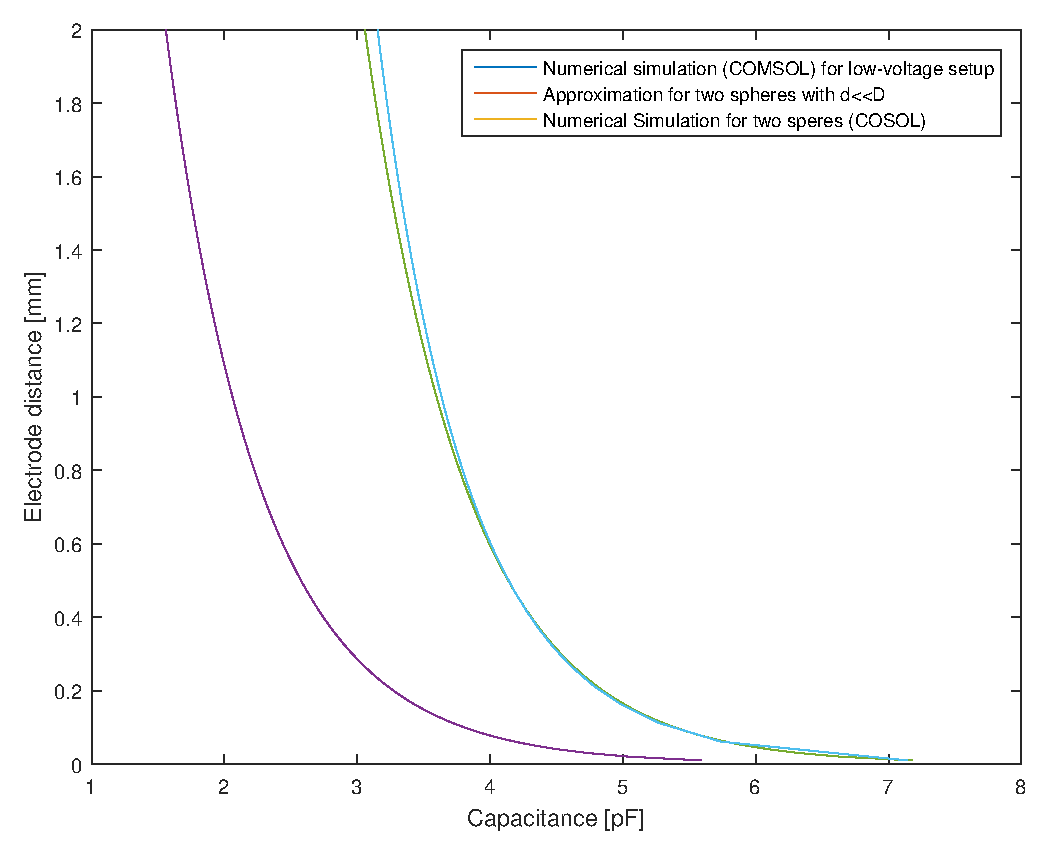
\includegraphics[scale=0.3]{figures/Comparison_Low_voltage_Two_spheres}		


	\caption[Kurze Abbildungsbeschreibung]{Dependency of the electrode distance on the capacitance for the low voltage setup and two spheres $\epsilon = 3.5$ }%

	\label{fig.waveforms}
\end{figure}

\section{Complex effective permittivity}
\subsection{}

\section{Performance of integrator}

\section{Dielectric Spectroscopy}

\begin{figure}[htbp]
\centering
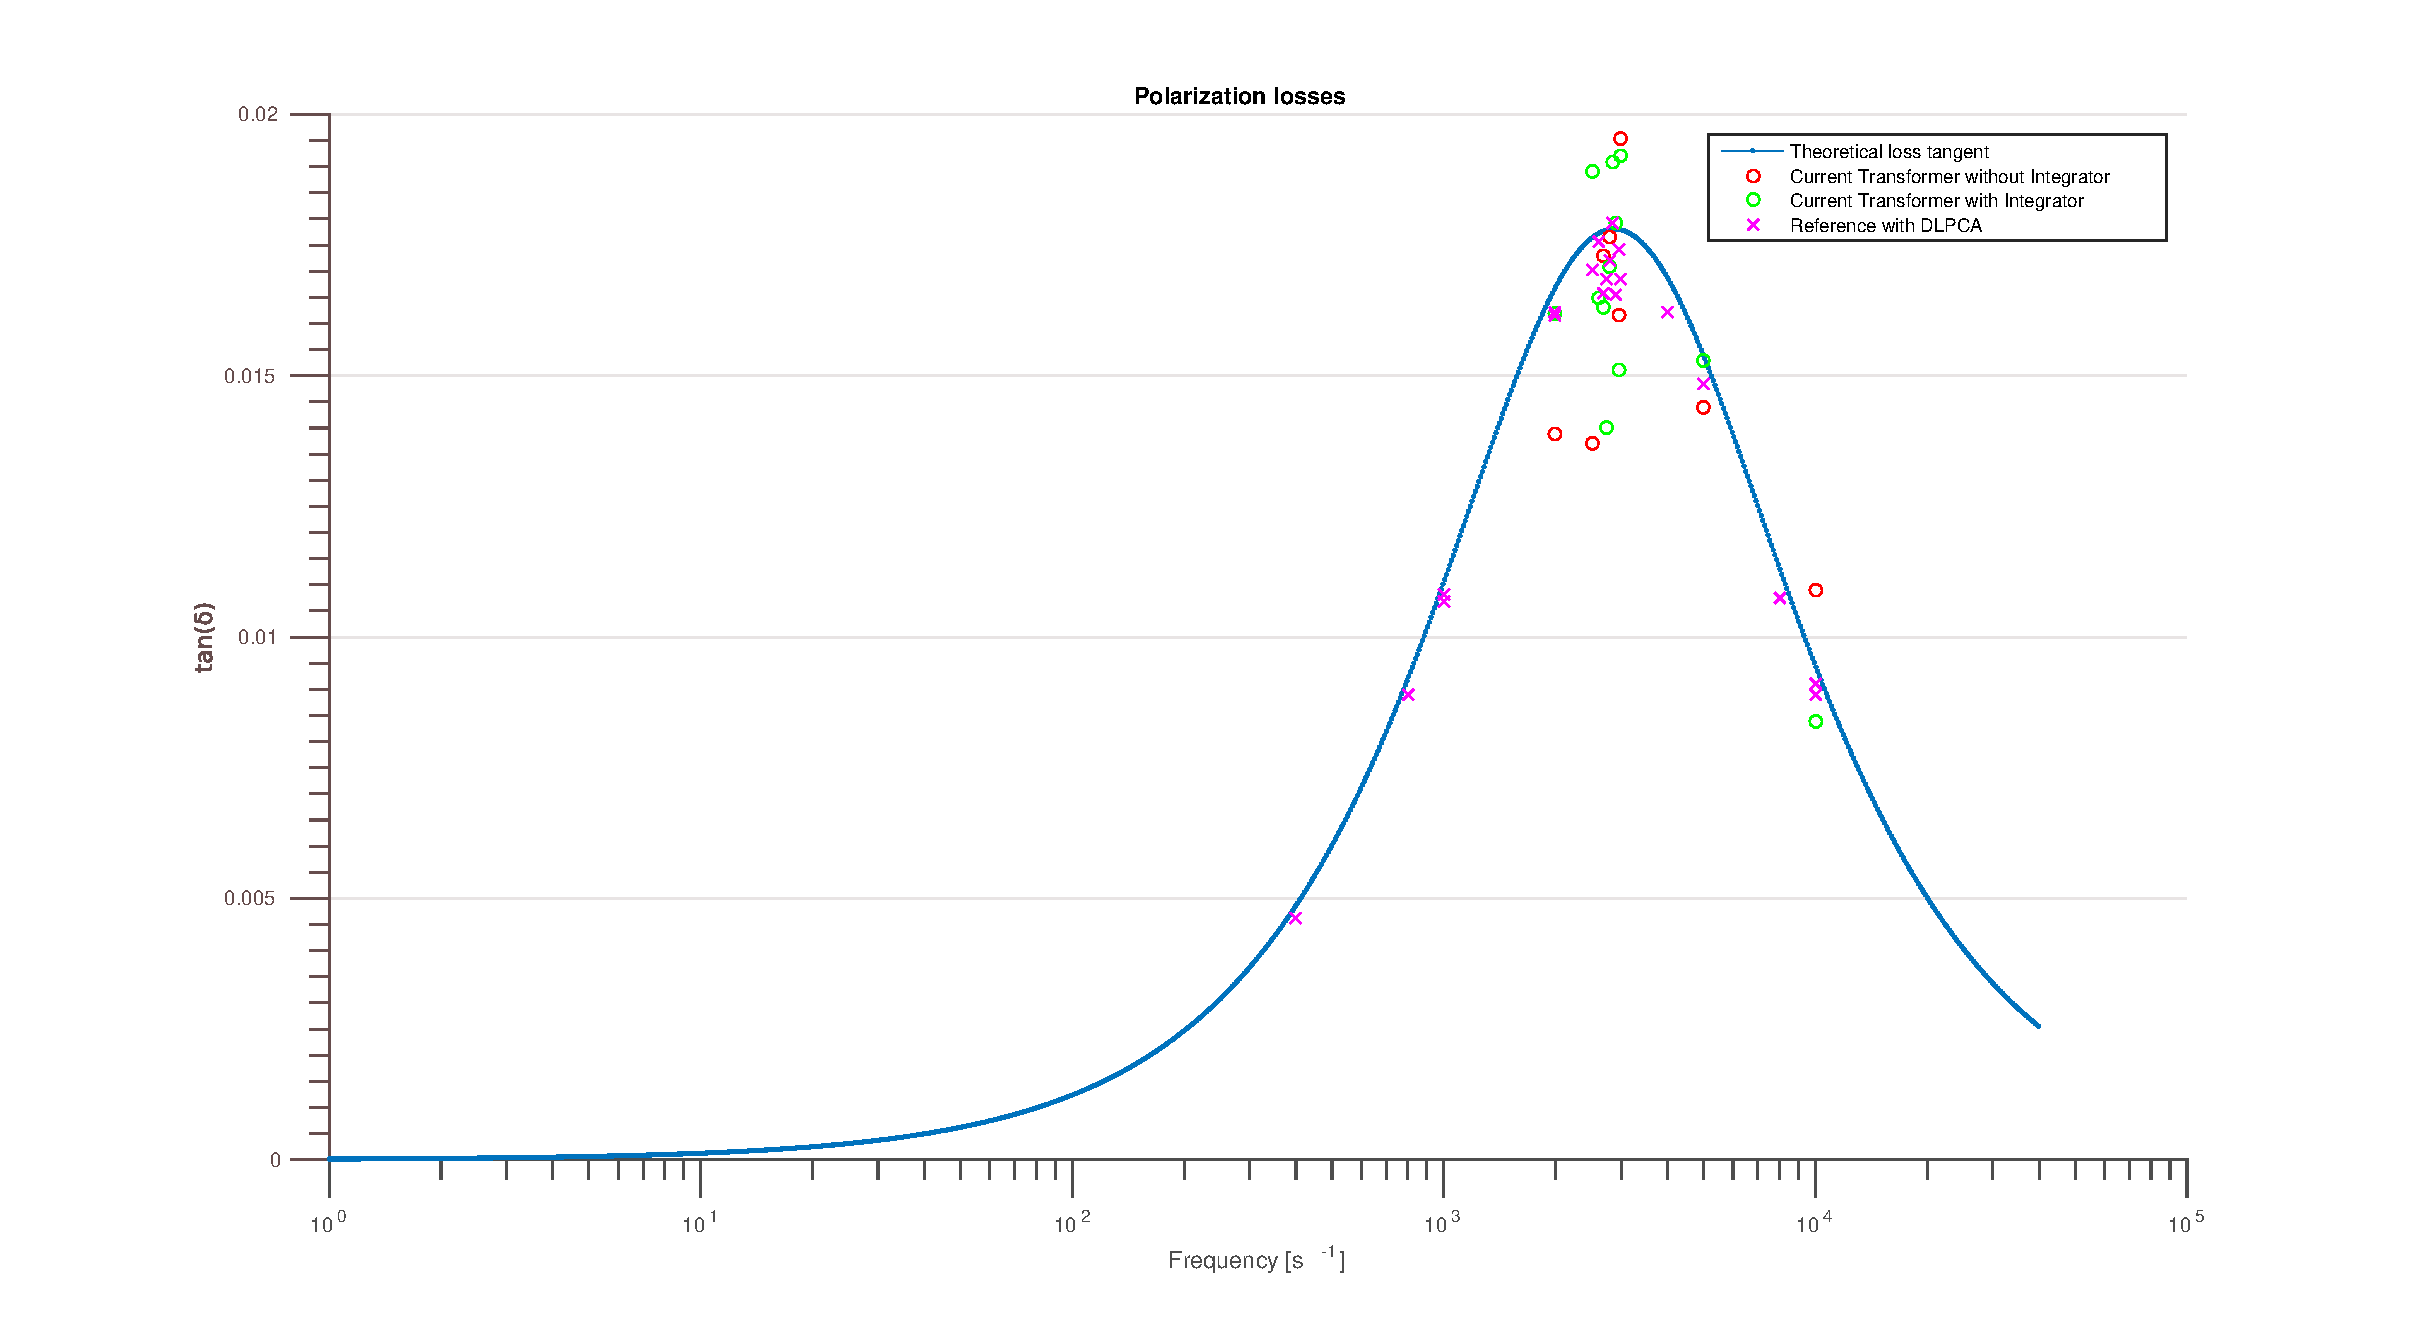
\includegraphics[scale=0.3]{figures/Results/Spectroscopy/spectroscopywithoutbars}
\caption[Kurze Abbildungsbeschreibung]{Measurements of dielectric loss tangent in different setup configurations}

\label{fig.spectroscopy}

\end{figure}
The three data series created from the spectroscopy experiment using the Debye model are shown in the graph above. The solid blue line represents the theoretical  dielectric loss tangent given the parameters of the components in the debye model
as a function of the frequency.
The components were assumed to be ideal and not to be temperature dependent.
The magenta data points can be used as a reference to evaluate the performance of the current transformer as these measurement points
were obtained with a industry standard low-noise current amplifier (DLPCA). 
The red points were recieved by replacing the DLPCA with the current transformer.
The green points were measured with the integrator in place, effectively integrating the voltage signal generated by the current transformer.
\newpage
\begin{figure}[htbp]
 \centering
 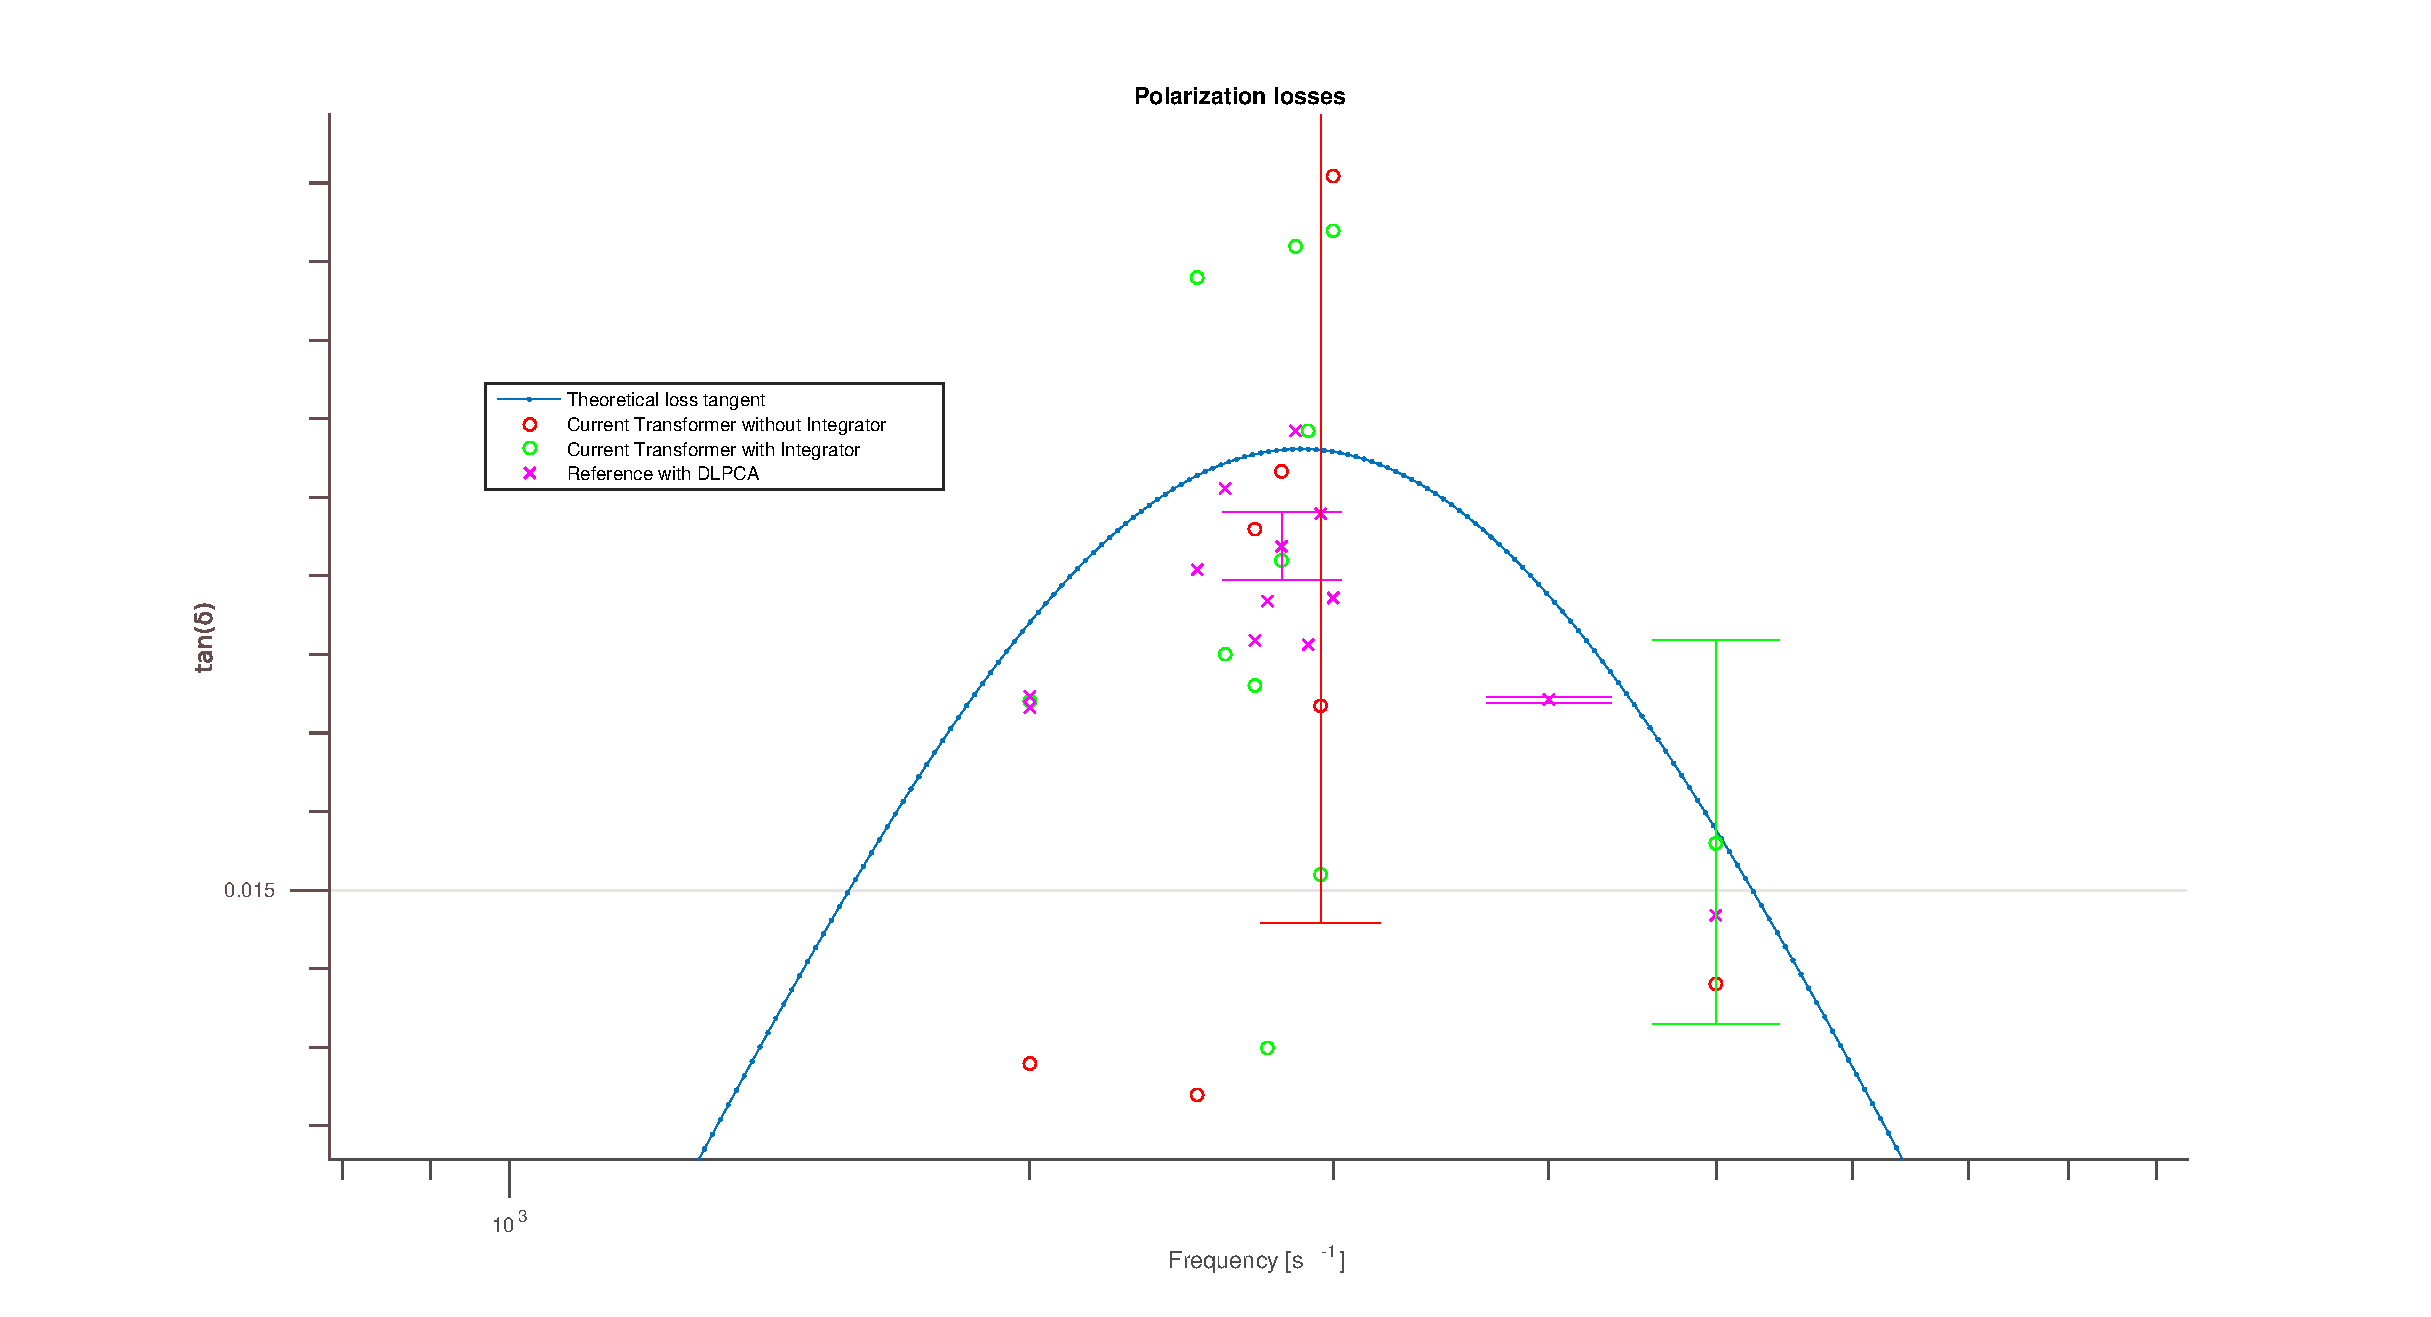
\includegraphics[scale=0.3]{figures/Results/Spectroscopy/errorbarsbettercolor}

\caption[Kurze Abbildungsbeschreibung]{Confidence intervals}
\label{fig.spectroscopy2}
\end{figure}

In order to adequately analyze the data points, the above graphic shows the previous plot
zoomed in around the maximum loss tangent since the deviation from the theoretical result seem to be the largest here.
The confidence intervals were added for a few points in each measurement series.

First it can be noted that while the reference measurements fit the curve the closest, the theoretical values are still not
within the measurements confidence intervals and the error can be greater than 10\%. To sum up the measurements conducted with
the current transformer, it can be stated that the measurement performance was significantly worse than the reference. Not only do they deviate further from the theoretical values
but they also have a larger variance. Which means that one cannot consistently predict a reasonable range for the mean of said measurement, at least not for only 9 phase averages.
While the use of the integrator succesfully lowered the deviation and shrinked the confidence intervals by a factor of 2 to 3, the measurement accuracy is still nowhere close to the one obtained with the DLPCA.

\subsection{Analysis of Noise Parameters}

In order to identify one of the sources to which the errors can be attributed, the noise level at the input and at the ouput was measured and analyzed to gain an estimation about how much noise was added in the system.
Using the current transformer in both configurations, i.e. with and without the integrator, the following parameters were measured. 

\newpage

\textit{Data without integrator:}
\begin{center}
\begin{tabular}{|m{3cm}|m{3cm}|m{1cm}|m{4cm}|m{2cm}|} 
\hline
frequency [Hz]& SNR & SNR & Noise Figure [dB] & Noise Floor \\ 
\hline \hline
2000 & 2.40E+07 & 16.31 & \cellcolor{blue!25}61.79 & 1.00E-05 \\ 
\hline
2500 & 1.8E+07 & 25.69 & \cellcolor{blue!25}58.55 & 1.00E-05 \\ 
\hline
2700 & 5.10E+07 & 31.02 & \cellcolor{blue!25}42.23 & 1.00E-05 \\ 
\hline
3000 & 5.13E+05 & 42.04 & \cellcolor{blue!25}40.86 & 1.00E-05 \\ 
\hline
5000 & 7.17E+06 & 79.386 & \cellcolor{red!25}49.56 & 1.00E-05 \\ 
\hline
10000 & 1.09E+06 & 377.35 & \cellcolor{red!25}34.616 & 1.00E-04 \\ 
\hline

\end{tabular}
\end{center}


\textit{Data with integrator:}
\begin{center}
\begin{tabular}{|m{3cm}|m{3cm}|m{1cm}|m{4cm}|m{2cm}|} 
\hline
frequency [Hz]& SNR & SNR & Noise Figure [dB] & Noise Floor \\ 
\hline \hline
2000 & 2.40E+07 & 16.31 & \cellcolor{blue!25}61.79 & 1.00E-05 \\ 
\hline
2500 & 1.8E+07 & 25.69 & \cellcolor{blue!25}58.55 & 1.00E-05 \\ 
\hline
2700 & 5.10E+07 & 31.02 & \cellcolor{blue!25}42.23 & 1.00E-05 \\ 
\hline
3000 & 5.13E+05 & 42.04 & \cellcolor{blue!25}40.86 & 1.00E-05 \\ 
\hline
5000 & 7.17E+06 & 79.386 & \cellcolor{red!25}49.56 & 1.00E-05 \\ 
\hline
10000 & 1.09E+06 & 377.35 & \cellcolor{red!25}34.616 & 1.00E-04 \\ 
\hline

\end{tabular}
\end{center}
	%
	\chapter{Discussion}

\section{Measures to improve the integrator}
The results indicate that the integrator has much noise at low frequencies. One might think that this does not influence the results as frequencies below 1kHz are not monitored, but this due to the spectral leakage of the FFT not the case.  A high-pass filter at the output of the integrator could reduce these parasitic frequency components. This might reduce the measured swing at the output of the integrator and thus improve the results of the dielectric spectroscopy. 
Moreover, a more detailed analysis of the origin of these low-frequency components is necessary. It has already been shown that the external voltage source is not responsible for them, thus the integrator has to be investigated part by part in order to find the origin of this noise. 
It would also be interesting to evaluate the transfer function of the integrator. Since the integrator has a gain of 80 dB the input power has to be chosen very low in order to stay within the allowed input power area of the network analyzer. Finally, the input is so low that the integrator does add too much noise, what makes an identification of the transfer function impossible. For a proper evaluation of the transfer function an amplifier / attenuator is necessary. 

Another measure to reduce the offset actively is a feedback loop. A PI-controller in the feedback loop at the output can make sure that there an offset at the input is erased as described in \cite{thomas}. 

\section{Measures to improve the current transformer}
As shown in the chapter \ref{chp.results} the measurements with the current transformer deteriorates the confidence interval of the measured $tan(\delta)$ by orders. This deterioration is reduced by the integrator, but it is still higher than with a shunt resistor. 
Furthermore, a more detailed analysis of the correlation between the NF of the current transformer (with and without integrator) for different frequencies and the confidence interval of the measured $tan(\delta)$ is necessary. This would provide detailed information what impact the quality of the current transformer has on the precision of the dielectric spectroscopy. 
The error class of the used Pearson CT 2877 is $+1 / -0 \% $, which includes current and phase errors as well as well as effects of harmonics in the primary current according to IEC 600-44-1. The phase shift errors of the CT 2877 are given by its Application Note {\url{http://www.pearsonelectronics.com/pdf/Application_20Notes.pdf} as below 6 degrees for frequencies at least one decade above the cutoff frequency. As 1 kHz is not one decade above the the corner frequency of 300 Hz it is not possible to make a serious guess which influence the phase shift caused by the current transformer has on the dielectric spectroscopy. There are as well CTs with lower corner frequencies below 300 Hz, which might result in lower phase errors. As the upper cutoff frequency is in the MHz area for all of them it is in general no problem to have a lower upper cutoff frequency. 

\section{Measures to improve the Debye model}
As shown in the results the measurements for the dielectric spectroscopy the theoretical $tan(\delta)$ is not within the confidence interval when measured with the DLPCA. This indicates that there are further parasitic impedances in the Debye model that were not considered. These might be prevented by evaluating the impedance with a network analyzer. 

	%
	\chapter{Conclusions}
\section{Estimation of current $\epsilon$}
The created lookup-table makes an estimation of the the electrode distance d possible.  Whin the chapters other factors than the air gap can be neglected . The correction factor of approx. to estimate the $\epsilon$ based on $\epsilon_eff$ improves the guess of $\epsilon$. Thus, within the range of the created look-up table the aims of this part of the semester project were reached. 

It has to be noted that this method is based on the assumption that the initial $\epsilon$ is always the same. This work did not investigate to what extend this assumption is tenable. 

\section{Statement on the suitability of the current transformer for dielectric spectroscopy}

The number of measurements for the polarization losses is quite low therefore it would be useful to increase the number of input frequencies in order to validate whether the measured values approximately possess the shape of the function of tan($delta$) over a larger area and how large the deviation from the theoretical value is. This necessitates an automation of the gain adaptation for the Butter worth amplifiers in order to use the resolution scope of the ADC ($\pm 10V$)  effectively. 
The band of the confidence interval for conduction losses is approx. 48 \% of the midpoint's value. This indicates that the noise level is too large to make a serious guess on the range of the 







%%%%%%%%%%%%%%%%%%%%%%%%%%%%%%%%%%%%%%%%%%%%%%%%%%%%%%%%%%%%%%%%%%%%%%%%%%%%%%%%
%Verzeichnisse
%%%%%%%%%%%%%%%%%%%%%%%%%%%%%%%%%%%%%%%%%%%%%%%%%%%%%%%%%%%%%%%%%%%%%%%%%%%%%%%%

	\bibliographystyle{alpha} %sagt, wie das Literaturverzeichnis dargestellt und geordnet wird
%	\bibliographystyle{geralpha} % fuer entsprechende deutsche Bezeichnungen im Literaturverzeichnis wie bspw 'Seite' statt 'page'
	\bibliography{Literature} 	%hier muss der Name des .bib Files eingegeben werden aus dem Latex die Bibliographiedaten lesen soll

%%%%%%%%%%%%%%%%%%%%%%%%%%%%%%%%%%%%%%%%%%%%%%%%%%%%%%%%%%%%%%%%%%%%%%%%%%%%%%%%
%Anhaenge
%%%%%%%%%%%%%%%%%%%%%%%%%%%%%%%%%%%%%%%%%%%%%%%%%%%%%%%%%%%%%%%%%%%%%%%%%%%%%%%%

	\appendix
%	\input{text/TechnischeZeichnungen}

	\input{text/Declaration of Orginality}

\end{document}
